\documentclass[crop,tikz]{standalone}

\usetikzlibrary{
    chains,
    positioning,
    arrows.meta,
    decorations.pathreplacing,
    calc,
    fit,
    shapes.geometric
}

\begin{document}

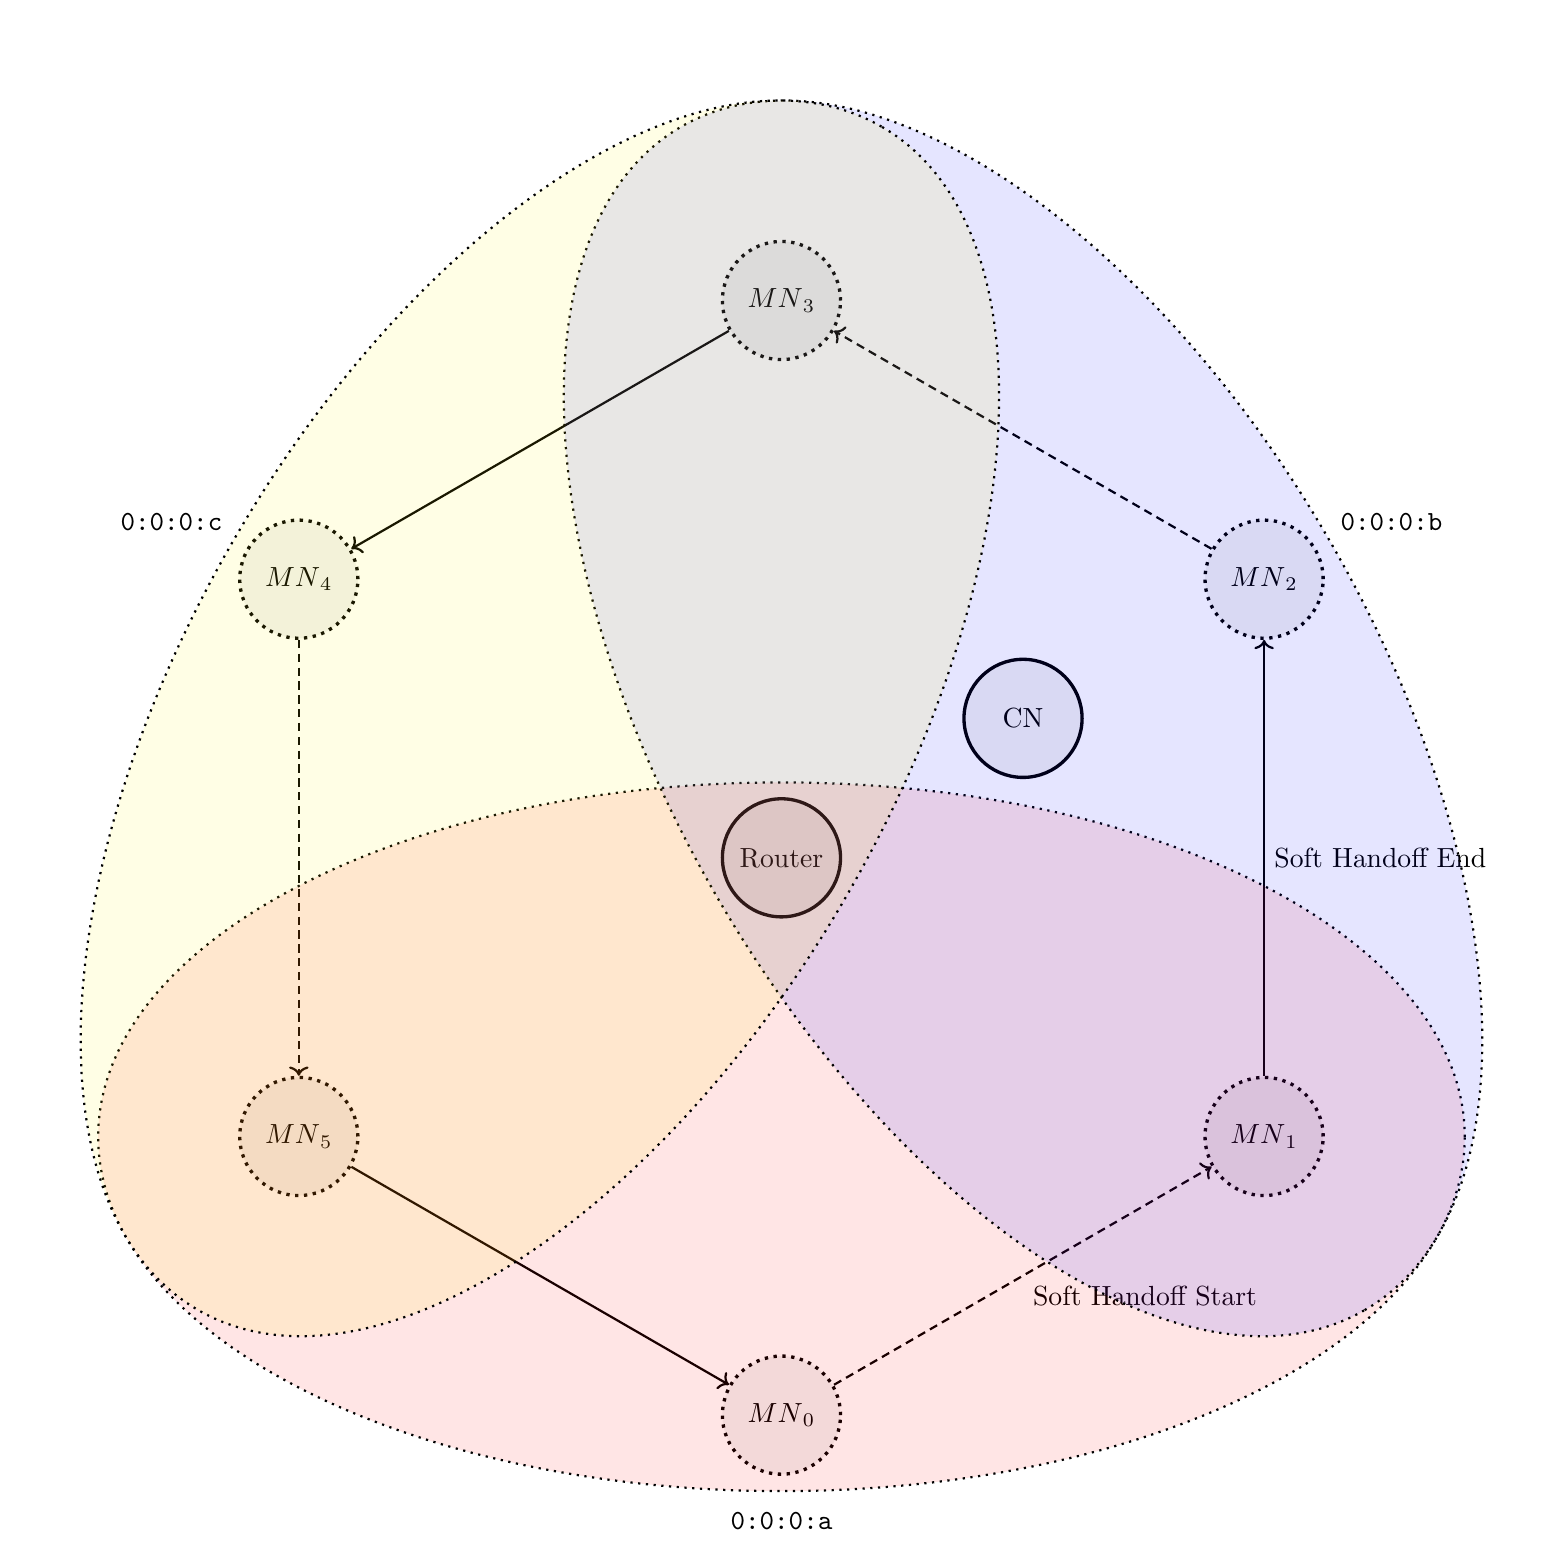
\begin{tikzpicture}[
    nwknode/.style={
        circle,
        very thick,
        minimum size=1.5cm,
        draw,
        fill=black!5,
    },
    network/.style args = {#1}{
        fit=(a.corner 2) (a.corner 3), 
        draw,
        ellipse,
        minimum height=9cm,
        inner xsep=0mm, 
        inner ysep=3mm,
        thick,
        dotted,
        fill=#1,
        fill opacity=0.1,
        text opacity=1,
        % 
    }
]
    \node[regular polygon, regular polygon sides=3, inner sep=2.5cm] (a) {};
    \node[regular polygon, regular polygon sides=6, inner sep=5cm]   (b) {};
    
    \node[nwknode, dotted] (mn0) at (b.side 4) {$\text{MN}_0$};
    \node[nwknode, dotted] (mn1) at (b.side 5) {$\text{MN}_1$};
    \node[nwknode, dotted] (mn2) at (b.side 6) {$\text{MN}_2$};
    \node[nwknode, dotted] (mn3) at (b.side 1) {$\text{MN}_3$};
    \node[nwknode, dotted] (mn4) at (b.side 2) {$\text{MN}_4$};
    \node[nwknode, dotted] (mn5) at (b.side 3) {$\text{MN}_5$};
    \node[nwknode] (cn)  at (a.side 3) {CN};
    
    \draw[->, thick, densely dashed] (mn0) -- node[below right] {Soft Handoff Start} (mn1);
    \draw[->, thick] (mn1) -- node[right] {Soft Handoff End} (mn2);
    \draw[->, thick, densely dashed] (mn2) -- (mn3);
    \draw[->, thick] (mn3) -- (mn4);
    \draw[->, thick, densely dashed] (mn4) -- (mn5);
    \draw[->, thick] (mn5) -- (mn0);
    
    \node[nwknode] (router) at (a) {Router};
    
    \node[network={red}, label={[anchor=south,above=-6mm]270:\texttt{0:0:0:a}}] {};
    \node[network={blue}, rotate=-60, label=\texttt{0:0:0:b}] at (a.side 3) {};
    \node[network={yellow}, rotate=60, label=\texttt{0:0:0:c}] at (a.side 1) {};
\end{tikzpicture}

\end{document}